%%&program=xelatex
%&encoding=UTF-8 Unicode
% SVN keywords
% $Author$
% $Date$
% $Revision$
% $URL$
\documentclass[a4paper,12pt]{article}      
%
\usepackage{ifxetex}% for XELATEX, or PDFlatex
\usepackage{ifplatform} 
\usepackage{empheq}
%
\ifxetex
	\usepackage{polyglossia} \setmainlanguage{portuges}
	\usepackage{fontspec}
	\ifwindows
		\setmainfont[Ligatures=TeX]{Garamond}
		\setsansfont[Ligatures=TeX]{Gill Sans MT}
		\setmonofont[Scale=MatchLowercase]{Courier}
	\fi
	\iflinux
		\setmainfont[Ligatures=TeX]{Linux Libertine O}
		\setsansfont[Ligatures=TeX,Scale=MatchLowercase]{Linux Biolinum}
		\setmonofont[Scale=MatchLowercase]{Courier}
	\fi
	\ifmacosx
	% add settings
	% Use xelatex -no-shell ...
	\fi
	\usepackage{xcolor,graphicx} 
\else
	\usepackage[portuguese]{babel}
	%\usepackage[latin1]{inputenc}
	\usepackage[utf8]{inputenc}
	\usepackage[T1]{fontenc}
	\usepackage{graphics}                 % Packages to allow inclusion of graphics
	\usepackage{color}                    % For creating coloured text and background
\fi

%\usepackage{hyperref}                 % For creating hyperlinks in cross references
\usepackage{enumitem}
\setlist{nolistsep}

\usepackage{amsmath,amssymb,amsfonts} % Typical maths resource packages
\usepackage[retainorgcmds]{IEEEtrantools}
\usepackage{caption}


\oddsidemargin 0cm
\evensidemargin 0cm

\pagestyle{myheadings}         % Option to put page headers
                               % Needed \documentclass[a4paper,twoside]{article}
\markboth{{\small \it  Laboratório de Física Experimental Básica}}
{{\small\it MEFT - 2013/2014} }

\addtolength{\hoffset}{-0.5cm}
\addtolength{\textwidth}{2.5cm}
\addtolength{\topmargin}{-1.5cm}
\addtolength{\textheight}{3cm}

%\textwidth 15.5cm
%\topmargin -1.5cm
\setlength{\parindent}{0pt}
\setlength{\parskip}{1ex  plus  0.5ex  minus  0.2ex}
%\textheight 25cm


% Math macros
\newcommand{\ud}{\,\mathrm{d}} 
\newcommand{\HRule}{\rule{\linewidth}{0.5mm}}

\author{Prof. Bernardo B. Carvalho} 
%%%%, Bernardo Brotas Carvalho\\bernardo@ipfn.ist.utl.pt} 
\date{ Outubro 2012} 

\begin{document} 

	
\includegraphics[width=0.2\textwidth]{../logo-ist}%\\[1cm]  %%  Logo_IST_color

	\HRule \\[0.5cm]
	{ \huge \sf  \textsc{Interferência e Difração de Ondas Eletromagnéticas num meio dielétrico, homogéneo e isotrópico .}} \\[0.4cm] % \bfseries 
%	{ \huge \sf  \textsc{Construções Geométricas em Lentes Delgadas (aproximação paraxial)} }\\[0.4cm] % \bfseries 
%	{ \large \bfseries Poder Dispersivo do Vidro. Poder de Resolução.}\\
%	{ \large \bfseries Procedimento Experimental}\\
	\HRule \\%[0.5cm]


%\title{Interferência e Difração de Ondas Eletromagnéticas num meio dielétrico, homogéneo e isotrópico } 

%\subtitle{ aplicação à luz visível} 
%\author{Prof. Isabel Cabaço} 


\section{\sf Introdução}
\subsection{\sf Onda plana monocromática }

Uma onda plana e luz pode ser estabelecida com uma lente convergente esférica e uma fonte luminosa pontual ou uma lente lente convergente cilíndrica 
e uma fonte linear(e.g um filamento linear).  À escala do Laboratório a luz solar é também uma excelente aproximação da Onda Plana.
Se a fonte de luz tiver apenas uma comprimento de onda (ou côr) ela é \emph{monocromática}, ou de frequência única e constante.
O modelo da onda plana monocromática que se propaga numa direção $\vec{s}$, descreve o campo  eletromagnético $\vec{E}$, $\vec{B}$ de acordo com
\footnote{A quantidade $e^{ i (\vec{k} \cdot \vec{r} -wt - \delta_0)}$ é apenas uma extensão matemática no conjunto complexo, $\mathbb{C}$,  que irá facilitar as contas de somar e, sobretudo, multiplicar. O campo Elétrico físico é dado pela \emph{componente real} deste número complexo. Chamemos $\mathbb{E}$ à extensão Complexa do vetor  $\vec{E}$.}, 
\footnote{``Recordar''  a \emph{fórmula de Euler}: $e^{i \alpha} = cis(\alpha) = \cos(\alpha) + i \sin(\alpha)$} :

\begin{align}
	\vec{E}(\vec{r}, t) &= \vec{E}_0 \cos(\vec{k} \cdot \vec{r} -wt -\delta_0) \label{eq:1}\\
	&=  \Re \{ \mathbb{E} \} = \vec{E}_0 \cdot \Re \{ e^{ i (\vec{k} \cdot \vec{r} -wt - \delta_0)}\} 
\end{align}

Em que, $\vec{k}$, é o número de onda ou vetor de propagação $\vec{k} =\frac{2 \pi}{\lambda}   \vec{s} $, $(\vec{k} \cdot \vec{r} -wt -\delta)$ é a fase da onda no ponto $\vec{r}$ e instante $t$ e 
$\delta_0$, a fase na origem,  que consideremos nula no resto do texto.

Pode provar-se que: 
\begin{enumerate}
	\item $\vec{E}$, $\vec{B}$ e $\vec{s}$ formam um triedo direto de um produto externo.

	\item $\vec{E}$ e $\vec{B}$ definem o plano de onda, que é portanto transversal à direçao de propagação, $\vec{s}$.

\end{enumerate}


\subsection{\sf Onda Esférica monocromática }
A onda criada por uma fonte pontual que radia isotrópicamente em todas as direções é dada por:
%Vamos supor que os campos que atingem o ponto $P$ são do tipo onda esférica (equação \label{eq:odesf}) 
\begin{align}
	\vec{E} &=  \frac{E_{0}}{r} \cdot \Re \{ e^{ i (k r -wt )}\} \cdot \vec{s}_r  \label{eq:odesf0}
%	E_2 &= E_{F_2} \frac{1}{r_2} e^{ i (k r_2 -wt )} \label{eq:odesf1} 
\end{align}
A direção de propagação varia com a posição e é radial $\vec{s}_r = \vec{r}/r$. A amplitude varia com $\frac{1}{r}$ e o termo espacial na fase é $k r$ (e não $ \vec{k} \cdot \vec{r} $ como na onda plana). 

\subsection{\sf Densidade de Energia na onda e Intensidade Luminosa}
\begin{enumerate}
\item A densidade de energia elétrica $w_e= \frac{\varepsilon |\vec{E}|^2}{2}$ é igual a
$w_m= \frac{ |\vec{B}|^2}{2\mu}$, $\varepsilon |\vec{E}|^2 = \frac{ |\vec{B}|^2}{2\mu}$, $\vec{B} = \sqrt{\varepsilon \mu} \vec{E}$, e
	 \begin{equation}
		\vec{B} = \mu \vec{H} \to \vec{H}= \sqrt{\frac{ \varepsilon}{\mu}} \vec{E} 
	\end{equation}
	\item A transferência de energia que acompanha a propagação da onda é descrita pelo vetor de Poynting 
	\begin{equation}
		\vec{S} = \vec{E} \times \vec{H} = \sqrt{\frac{ \varepsilon}{\mu}} |\vec{E}|^2 \vec{s} 
	\end{equation}
	$ \vec{s}$ é a direção em que se propaga a onda e a energia.
	
	O fluxo do vetor de Poynting representa a energia que na unidade de tempo atravessa a superfície fechada (que delimita um Volume) perpendicularmente a ela. Porque a energia se conserva é igual à diminuição no tempo de energia no interior do Volume considerado.
	O vetor de Poynting é assim a quantidade de energia que flui por unidade de tempo e por unidade de área (e perpendicularmente a ela) 
	 
	\item A intensidade luminosa ou radiância é calculada pelo valor médio (no tempo: “$\langle \, \rangle$”) do módulo do vetor de Poynting: 
	\begin{equation}
		I = \langle S \rangle = \sqrt{\frac{ \varepsilon}{\mu}} \langle |\vec{E}|^2 \rangle \label{eq:5} 
	\end{equation}
	A partir da equação (\ref{eq:1}) e sabendo-se que  $\langle (A \cos(wt) )^2  \rangle =\frac{1}{2} A^2$,  obtém-se 
	\begin{equation}
		\label{eq:6} I = \frac{1}{2}\sqrt{\frac{ \varepsilon}{\mu}} |\vec{E}|^2 
	\end{equation}
	e usando a representação complexa: 
	\begin{equation}
		\label{eq:7} I = \frac{1}{2}\sqrt{\frac{ \varepsilon}{\mu}}  \mathbb{E}\, \mathbb{E}^* 
	\end{equation}
	em que $\mathbb{E}^*$ é o \emph{complexo conjugado} de $\mathbb{E}$, i.e. se $\mathbb{E} = \vec{E} \cdot e^{ \alpha} \to \mathbb{E}^* = \vec{E} \cdot e^{- \alpha}$.
\end{enumerate}

%***********************
\section{\sf Interferência de ondas eletromagnéticas produzida por duas fontes coerentes afastadas entre si de $\underline{a}$ }
\begin{figure}[h!tb]
	\centering 
	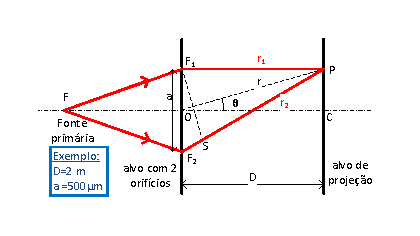
\includegraphics[width=0.8
	\textwidth]{interf} \caption{Interferência produzida por duas fontes coerentes. As dimensões NÃO estão à escala, na realidade tem de se ter $D \gg a$. \label{fig:1}} 
\end{figure}

Se um feixe de luz incidir em duas fendas, então do lado direito é como se tivermos duas fontes pontuais situadas nas posições $F_1$ e $F_2$.

Se distâncias $F F_1 = F F_2$ as amplitudes e as fases do campo $E$ em $F_1$ e $F_2$ são idênticas e as fontes são coerentes\footnote{De forma a que o atraso entre os dois raios não fosse maior que o \emph{tempo de coerência da fonte}}.
%, i.e. desde que a diferença de fase entre os dois centros fosse bem definida e constante).
%(mesmo se a distância de percurso não fosse a mesma continuariam coerente, se a distância de percurso não fosse excessiva

Em qualquer ponto do alvo de projeção a soma é vetorial: 
\begin{equation}
	\label{eq:8} \vec{E}_{total} = \vec{E}_1 + \vec{E}_2  = \Re \{ \mathbb{E}_1 + \mathbb{E}_2 \} 
\end{equation}
em que $\vec{E}_i$ é o campo elétrico devido à fonte $F_i$

A intensidade (\ref{eq:7}) virá pois 
\begin{align}
	I &= \frac{1}{2}\sqrt{\frac{ \varepsilon}{\mu}} \; \langle \mathbb{E}_{total} \mathbb{E}^*_{total} \rangle \nonumber \\
	&= \frac{1}{2}\sqrt{\frac{ \varepsilon}{\mu}} \left[ \langle \mathbb{E}_1 \mathbb{E}^*_1 + \mathbb{E}_1 \mathbb{E}^*_2 + \mathbb{E}^*_1 \mathbb{E}_2 + \mathbb{E}_2 \mathbb{E}^*_2 \rangle \right] \nonumber \\
	&= I_1 + I_2 +I_{12} 
\end{align}

em que 
\begin{equation}
	\label{eq:10} I_1 =\frac{1}{2}\sqrt{\frac{ \varepsilon}{\mu}} \;  \langle \mathbb{E}_{1} \mathbb{E}^*_{1} \rangle \quad \text{,} \quad \text{e} \quad  I_2 =\frac{1}{2}\sqrt{\frac{ \varepsilon}{\mu}} \; \langle \mathbb{E}_2 \mathbb{E}^*_2 \rangle
\end{equation}
A intensidade total difere da soma das intensidades no termo $I_{12} $, chamado termo de interferência 
\begin{equation}
	\label{eq:11} I_{12} =\frac{1}{2}\sqrt{\frac{ \varepsilon}{\mu}} \; \langle \mathbb{E}_1 \mathbb{E}^*_2 + \mathbb{E}^*_1 \mathbb{E}_2 \rangle 
\end{equation}
mas os dois termos são conjugados um do outro 
\begin{equation}
	\label{eq:12} \mathbb{E}_1 \mathbb{E}^*_2 = (\mathbb{E}^*_1 \mathbb{E}_2)^* 
\end{equation}

Para calcular vamos supor que os campos que atingem o ponto $P$ são do tipo onda esférica (equação \ref{eq:odesf0}) 
\begin{align}
	E_1 &= E_{F_1} \frac{1}{r_1} e^{ i (k r_1 -wt )} \label{eq:odesf}\\
	E_2 &= E_{F_2} \frac{1}{r_2} e^{ i (k r_2 -wt )} \label{eq:odesf1} 
\end{align}
%as amplitudes variam com $\frac{1}{r}$ e o termo espacial na fase é $k r$ (e não $ \vec{k} \cdot \vec{r} $ como na onda plana). 

\begin{equation}
	\label{eq:15} \text{ como } F F_1 = F F_2 \, \to \, \quad E_{F_1} = E_{F_2} = E_{F} 
\end{equation}
Do esquema da fig. 1 pode concluir-se que 
\begin{equation}
	\label{eq:16} r_2 \approx r_1 + a \sin \theta 
\end{equation}
a quantidade $ a \sin \theta $ tem um valor muito pequeno\footnote{Esta quantidade quando comparada com $ r_1$: \; $ \frac{a \sin \theta }{r_1 } \sim \frac{a}{r } \sim \frac{ 500 \times 10^{-6} }{2 } \sim 10^{-4}$},
i.e. na amplitude dos campos em (\ref{eq:odesf}) e (\ref{eq:odesf1}) $ r_1 \cong r_2 = r$. 
Mas a mesma aproximação não pode ser feita na fase, porque em 
\begin{align}
	k r_2 &= k r_1 +k a \sin \theta  \nonumber \\ %\,\text{, e }
	k a \sin \theta &= \frac{ 2 \pi }{\lambda } a \sin \theta  \rightarrow \text{ varia entre } 0 \text{ e } \frac{ 2 \pi}{\lambda} a \sim 5 \cdot 10^{3} \text{, para }  \lambda \simeq 600\,nm  \nonumber 
\end{align}
produzindo variações muito sensíveis na fase. 
\begin{align}
	\label{eq:17} I_{12} &=\frac{1}{2}\sqrt{\frac{ \varepsilon}{\mu}} \left(E_{F} \cdot \frac{1}{r }\right)^2 \; \left[ \langle e^{ i (k r_1 -wt )} e^{ -i (k r_2 -wt ) } + \text{ conjugado} \rangle \right] \nonumber \\
	&= \frac{1}{2}\sqrt{\frac{ \varepsilon}{\mu}} \left(\frac{E_F}{r }\right)^2 \; \left[ \langle e^{ i k (r_1 - r_2) } + \text{ conjugado} \rangle \right] 
\end{align}
Atendendo à fórmula de Euler, o termo entre parêntesis retos  em (\ref{eq:17}) é 
\begin{equation*}
	2 \cos ( k (r_1 - r_2) ) = 2 \cos ( k (r_2 - r_1) ) = 2 \cos ( k a \sin \theta ) 
\end{equation*}
com a hipótese ( \ref{eq:15}) 
\begin{equation}
	\label{eq:18} I_1= I_2 = \frac{1}{2}\sqrt{\frac{ \varepsilon}{\mu}} (\frac{E_F}{r })^2 
\end{equation}
\begin{align}
	I_{12} &= 2 I_1 \cdot \cos ( k a \sin \theta ) \\
	I_{total} &= 2 I_1 \left[ 1 + \cos ( k a \sin \theta ) \right ] 
\end{align}
mas $ \cos X = \cos^2 \frac{X}{2} - \sin^2 \frac{X}{2} = 2 \cos^2 \frac{X}{2} - 1$ ; $ \cos X +1 = 2 \cos^2 \frac{X}{2}$
\begin{equation}
	\label{eq:21} I_{total} = 4 I_1 \cdot  \cos^2 (\frac{k a \sin \theta }{2} ) 
\end{equation}

\begin{figure}[h!tb]  \centering 
	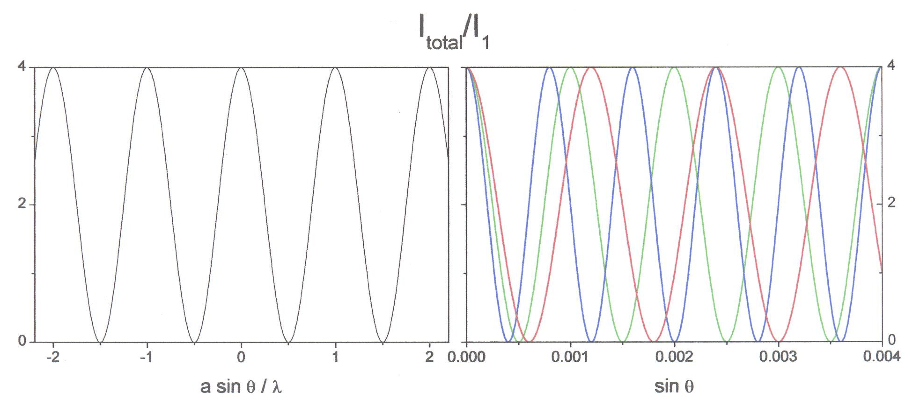
\includegraphics[width=\textwidth]{figura2} 
	\caption{Intensidade da figura de interferência produzida por duas fontes coerentes. Fonte monocromática (esquerda) e policromática (direita).\label{fig:2}} 
\end{figure}


Ver representação gráfica na fig. \ref{fig:2}. A função da expressão (\ref{eq:21}) está representada à esquerda para uma fonte monocromática.
Apresenta máximos para: $ \cos^2 \left( \frac{k a}{2} \sin \theta \right)= 1 $, ou seja:
\begin{align}
	\text{ máximos para }\frac{k a}{2} \sin \theta &= m \pi \label{eq:22} \\
	\text{ e mínimos para } \frac{k a}{2} \sin \theta &= (2m +1)\frac{\pi}{2} \label{eq:23} 
\end{align}

Os máximos de intensidade correspondem a: 
\begin{empheq}[box=\fcolorbox{blue!40!black!60}{yellow!20}]{equation}
%\framebox[4cm][c]{
%\begin{equation}
	 \sin \theta = \frac{m \lambda}{a}  \label{eq:maxDF}
%\end{equation}
%}
\end{empheq}

São igualmente afastados no eixo  $\sin \theta$ e têm teoricamente a mesma intensidade, sendo o máximo de ordem zero observado no ponto central (C na figura \ref{fig:1} )

$m$ é a \emph{ordem de interferência} e corresponde ao número de comprimentos de onda (c.d.o.) de que diferem os percursos, $r_1$ e $r_2$, no ponto considerado (por exemplo para $|m|=2$,  $r_1$ e $r_2$ diferem de $2\lambda$). 

Na relação (\ref{eq:maxDF}), $\sin \theta$  varia linearmente com $\lambda$. Na figura \ref{fig:2} à direita, representa-se a figura de interferência para uma radiação policromática\footnote{$\lambda_{azul} = 400nm,\; \lambda_{verde} = 500nm,\; \lambda_{vermelho} = 600nm,\; a= 50\, \mu m$}. Só na ordem zero há coincidência dos máximos. O $1^{\circ}$ máximo de ordem $1$ é \emph{irisado}. Para ordens elevadas a mistura de várias ordens dará um ``branco sujo''.

%1\textdegree{}'

%***********************
\section{ \sf Difração por uma Fenda}
\label{sec:fenda} 
As primeiras interpretações das figuras de difração foram feitas por Huygens e Fresnel que supuseram que os pontos de um écran, com uma fenda iluminada por uma fonte luminosa $F$, constituem fontes secundárias que emitem ondas esféricas que interferem entre si. A dedução que se apresenta é válida quando a maior das distâncias $r$ entre $F$ e um ponto da fenda $O$ ou $OQ$ (sendo $Q$ um ponto do alvo de projeção) é tal que $\frac{r}{s} \gg \frac{s}{\lambda}$, em que $s$ é a largura da fenda e $\lambda$ o comprimento de onda emitido por $F$. Esta aproximação é conhecida como {\bf aproximação de Fraunhofer} e corresponde a considerar que $F$ emite uma onda que, quando atinge a fenda, é praticamente uma onda plana.

\begin{figure}[tb]  \centering 
	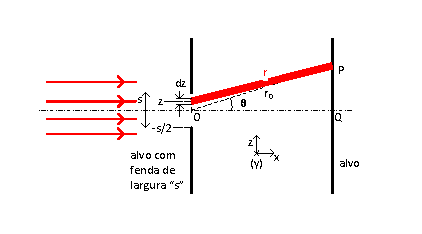
\includegraphics[width=0.9\textwidth]{fenda} 
	\caption{Difração produzida por uma fenda. As dimensões não estão à escala ($r \gg s$).\label{fig:3}} 
\end{figure}

A contribuição do elemento $\ud z$ do écran (à distância $z$ da origem) para o campo elétrico em $P$ é elementar e é 
\begin{equation}
	\label{eq:25} dE_P(\ud z) = \frac{E(z)}{r(z)} e^{i(kr- wt)} \ud z 
\end{equation}

em que $E(z)$ é a amplitude do campo no ponto médio do elemento $dz$ e $r(z)$ é a distância deste ponto a $P$.

Em 1ª aproximação (dado que $s \ll r;\; s \simeq 10^2 \mu m$, $r \sim 1m$ ) 
\begin{equation}
	\label{eq:26} r(z)= r_0 - z \sin \theta 
\end{equation}
Em que o termo $z \sin \theta $ é muito inferior a $r_0$

O cálculo de $E_P$ é feito somando todas as contribuições do tipo (\ref{eq:25}) 
\begin{align}
	E_P &= \int_{-\frac{s}{2}}^\frac{s}{2} \ud E_P = \int_{-\frac{s}{2}}^\frac{s}{2} \frac{E(z)}{r(z)} e^{i (k r_0 - k z \sin \theta -w t) } \ud z \nonumber\\
	&= ( \frac{E}{r} )_{z=0}\; e^{i (k r_0 -w t) } \int_{-\frac{s}{2}}^\frac{s}{2} e^{ -i k z \sin \theta } \ud z 
\end{align}

$E(z) \simeq E(z=0) $ na hipótese da onda plana que atinge o écran.\\
$r \simeq r(z=0) = r_0 $ na amplitude, aproximação que não é feita na fase.\\
O integral 
\begin{align} \label{eq:28}
	\int_{-\frac{s}{2}}^\frac{s}{2} e^{ -i k z \sin \theta } \ud z &= \frac{1}{-i k \sin \theta } \left[ e^{ -i k z \sin \theta } \right]_{-\frac{s}{2}}^\frac{s}{2}\nonumber \\
	&= \frac{1}{-i k  \sin \theta } \left[ e^{ -i k \frac{s}{2} \sin \theta } + e^{ +i k \frac{s}{2} \sin \theta } \right] 
\end{align}

Mas pela fórmula de Euler 
\begin{equation}
	\label{eq:29} \left[ \cdots \right] = -2 i \sin( \frac{k s}{2}\sin \theta) 
\end{equation}

%\hspace{1.0cm}
O integral virá pois igual a 
\begin{equation*}
	\frac{2 \sin( \frac{k s}{2}\sin \theta)}{  k \sin \theta}= s \; \frac{ \sin( \frac{k s}{2}\sin \theta)}{ \frac{k s}{2}\sin \theta} 
\end{equation*}
\begin{equation}
	\label{eq:30} E_P = \left( \frac{E}{r} \right)_{z=0} \; s  \;\frac{ \sin( \frac{k s}{2}\sin \theta)}{ \frac{k s}{2}\sin \theta}  \; e^{i(k r_0 -wt) }
\end{equation}

\begin{figure}[htb]  \centering 
	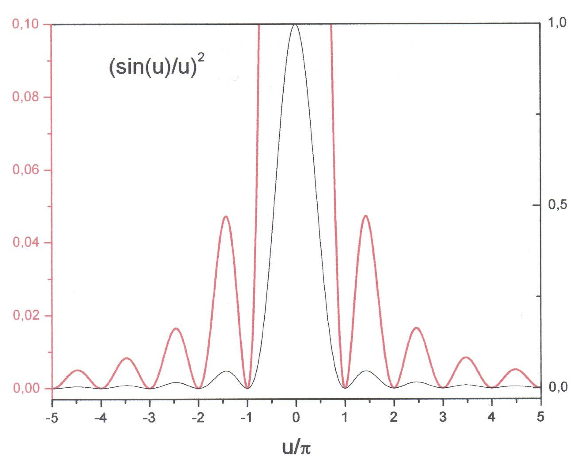
\includegraphics[width=0.7
	\textwidth]{figura4.png} \caption{
	Evolução da função $\left( \frac{\sin u}{u} \right)^2 $ (a preto). Para se visualizarem os máximos secundários apresenta-se a vermelho no mesmo gráfico com a escala de ordenadas ampliada de 10 vezes.
A mancha central tem uma extensão (em $\sin \theta$) que é dupla das manchas laterais. \label{fig:4}} 
\end{figure}

A intensidade $I(\theta)$ será pois
\begin{equation}
	\label{eq:31} I(\theta) = \frac{1}{2}\sqrt{\frac{ \varepsilon}{\mu}} \; \left( \frac{E}{r} \right)_{z=0}^2 \; s^2 \; \left[ \frac{ \sin( \frac{k s}{2}\sin \theta)}{ \frac{k s}{2}\sin \theta} \right]^2 
\end{equation}

O último termo $\left[ \cdots \right] $  é do tipo $(\frac{\sin u}{u})^2 $ (Figura \ref{fig:4}) e tem zeros para $u = m \pi$ com $m \neq 0$. Tem um máximo principal para $m = 0$ e vale $1$. Assim o fator $I_0 \equiv \frac{1}{2} \sqrt{\frac{ \varepsilon}{\mu}} (\frac{E}{r })_{z=0}^2 s^2$ representa o valor de intensidade máxima que se vai observar no ponto $Q$ (figura \ref{fig:3})
\begin{equation}
	\label{eq:32} I = I_0 \cdot \underbrace{\left( \frac{\sin u}{u} \right)^2}_\text{Fator de forma de fenda} \text{, com } u\equiv \frac{k s}{2}\sin \theta 
\end{equation}

\subsection{ \sf Mínimos da figura de difração de uma Fenda}
Os zeros de $(\frac{\sin u}{u})^2 $ correspondem a  
\begin{equation}
	\label{eq:33} \frac{k s}{2}\sin \theta = m \pi \text{, com } m \ne 0 \Rightarrow \frac{2 \pi}{\lambda} \frac{ s}{2} \sin \theta = m \pi
\end{equation}
 ou seja:
\begin{empheq}[box=\fcolorbox{blue!40!black!60}{yellow!20}]{equation}
	\sin \theta = m \frac{\lambda}{s} \text{, com } m \text{ inteiro }\ne 0 \label{eq:minF} 
\end{empheq}
[Notar são mínimos laterais e não máximos como na equação \ref{eq:maxDF}]
%\begin{equation}
%	\label{eq:34} \frac{2 \pi}{\lambda} \frac{ s}{2} \sin \theta = m \pi \Rightarrow \sin \theta = m \frac{\lambda}{s} 
%\end{equation}


$m= \pm 1 $ corresponde à posição do 1º mínimo que rodeia o máximo central e $\sin \theta_{m=1} = \frac{\lambda}{s}$\,.\\
 $\theta_1$ é o ângulo segundo o qual do centro da fenda se vê o 1º mínimo.

 Quanto  aos máximos da figura embora estejam situados naturalmente entre os vários mínimos, NÃO são dados, desta vez,   pela expressão do tipo (\ref{eq:23}). Como tal não consideremos as suas posições exatas neste trabalho 
 (contudo ver apêndice \ref{sec:maxfenda}).
% $\frac{k s}{2}\sin \theta = (2 m +1)\frac{\pi}{2} $ 

%%%%%%%%%%%%%%%%%%%%%%%%%
%\pagebreak[4] 
\section{\sf Difração por N Fendas de Largura \underline{$s$} \mbox{afastadas} de \underline{$a$}}

\begin{figure}
	[!tb]  \centering 
	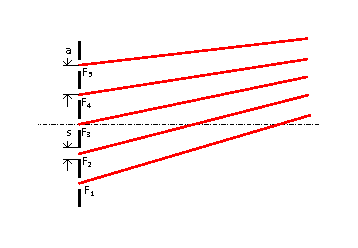
\includegraphics[width=0.8\textwidth]{Nfendas} \caption{Difração produzida por $N$ Fendas de Largura $s$ afastadas de $a$ \label{fig:Dif_N_s_a}} 
\end{figure}

\subsection{Primeiro, SEM considerar o efeito de largura da fenda, $s$}

Nesta aproximação considera-se que: $s\to 0$ (fontes pontuais).
 
As $N$ fendas são iluminadas por uma fonte luminosa tal que os valores do campo elétrico $\vec{E}_0$ nas diferentes aberturas são os mesmos em amplitude e fase (aproximação de onda plana). O campo elétrico total $\vec{E}_P$ num ponto $P$ do alvo de projeção vem:   
\begin{equation}
	\label{eq:dif_soma} \vec{E}_P = \vec{E}_{P_1} + \vec{E}_{P_2} +\cdots +\vec{E}_{P_N} 
\end{equation}
%\newpage 
em que $E_{P_i}$ representa a contribuição da fenda \underline{i} para o campo no ponto $P$ (ver Figura \ref{fig:Dif_N_s_a}). 
\begin{align}
	\label{eq:38} |\vec{E}_{P_1}| &= E_0 \frac{1}{r_1} e^{i(k r_1 -wt)} \nonumber \\
	|\vec{E}_{P_2}| &= E_0 \frac{1}{r_2} e^{i(k r_2 -wt)} \qquad r_2 = r_1 - a \sin \theta \\
	|\vec{E}_{P_j}| &= E_0 \frac{1}{r_i} e^{i(k r_i -wt)}\qquad r_j = r_1 - (j-1) a \sin \theta \nonumber 
\end{align}

O termo $((j-1) a \sin \theta) \ll r_1$ e pode desprezar-se na amplitude de $E_{P_j}$ mas terá que ser considerado na fase. A soma (\ref{eq:dif_soma} ) é: 
\begin{equation}
	\label{eq:39} E_{P} = \frac{E_0}{r_1} \; e^{i(k r_1 -wt)} \left[ \underbrace{1 + e^{-i k a \sin \theta} + e^{-i k 2 a \sin \theta} + \cdots + e^{-i k (N-1) a \sin \theta}}_{\text{N termos} }\right]
\end{equation}

Podemos reconhecer na expressão anterior uma soma de termos de uma progressão geométrica de razão $R = e^{-i k a \sin \theta}$, cuja soma 
é 
\begin{equation}
	\frac{1-R^N}{1-R} u_1  = \frac{1-e^{-i N X}}{1-e^{-i X}} = \frac{1-e^{-i N k a \sin \theta}}{1-e^{-i k a \sin \theta}} \label{eq:40}
\end{equation}


A Intensidade vem, de (\ref{eq:7}),  $I_P  =\frac{1}{2} \sqrt{\frac{ \varepsilon}{\mu}} E_P E_P^*$ 
\begin{equation}
	E_P E_P^* = (\frac{E_0}{r})^2 \cdot  \big[\text{soma} \big] \cdot \big[\text{ soma}^* \big] \label{eq:41}\\
\end{equation}

O produto dos fatores $ [\text{soma} ] \cdot [\text{ soma}^* ]$ é do tipo 

\begin{align}
\label{eq:42} 
 \left( \frac{1-e^{-i N X}}{1-e^{-i X}} \right) \cdot \left( \frac{1-e^{+i N X}}{1-e^{+i X}}  \right)  &= \nonumber\\
%\end{equation}
%
%	&\text{Com } X = k a \sin \theta \label{eq:43} 
%
%Que com  $X = k a \sin \theta$ obtém-se  % para (\ref{eq:40}) 
%\begin{align}
	 \frac{1-e^{-i N X}-e^{i N X}+1}{1-e^{-i X} -e^{i X} +1} &= \frac{2-(e^{-i N X}+e^{i N X})}{2-(e^{-i X} -e^{i X})} = \nonumber \\
	\frac{2- 2 \cos NX }{2- 2 \cos X} &= \frac{1- \cos NX }{1- \cos X} = \frac{2\sin^2 \frac{NX }{2} }{2\sin^2 \frac{X }{2}} = \frac{\sin^2 \frac{NX }{2} }{\sin^2 \frac{X }{2}} 
\end{align}


Que, com $v \equiv \frac{k a }{2} \sin \theta = \frac{X}{2}$, se obtém  % para (\ref{eq:40}) 
%  $X = k a \sin \theta$ obtém-se  % para (\ref{eq:40}) 

\begin{align}
	I_P &= \frac{1}{2} \sqrt{\frac{ \varepsilon}{\mu}} ( \frac{E_0}{r})^2 N^2 \left( \frac{\sin\frac{NX }{2} }{N \sin \frac{X }{2}} \right)^2 \nonumber \\
	&= I_0 \; \left( \frac{\sin N v }{N \sin v} \right)^2 \label{eq:45}
\end{align}

O termo $\big( \frac{\sin N v }{N \sin v} \big)^2$ designa-se termo de interferência e corresponde à \emph{interferência de $N$ fendas}.

\subsubsection{Máximos Principais}
Para $ v = m \pi$ temos 
\begin{equation*}
 \left.
	\begin{array}{rl} 
			\sin v =0 \\
			\sin Nv =0 \\			
	\end{array} \right\} 
  \Rightarrow \big( \frac{\sin N v }{N \sin v} \big)^2 \to \left( \frac{0 }{0} \right)^2 
\end{equation*}


%\Big( \frac{\sin N v }{N \sin  v} \Big)^2
\begin{equation}
	\label{eq:46} \lim_{v \rightarrow m \pi} \frac{\sin N v}{N \sin v} = \lim_{v \rightarrow m \pi} \frac{N \cos N v}{N \cos v} =\frac{N (\pm 1)}{N (\pm 1)} = \pm 1 
\end{equation}

Quando $v \rightarrow 0 \quad \lim (\cdots)^2  =  1$, %\\[5pt]
e portanto o fator que multiplica o termo de interferência na expressão (\ref{eq:45}) é  $I_0$, a intensidade no centro da figura  de interferência.

O termo de interferência terá uma série de \emph{máximos principais} laterais $ v = \frac{k a }{2} \sin \theta = m \pi$, ou seja

\begin{empheq}[box=\fcolorbox{blue!40!black!60}{yellow!20}]{equation}
	 \sin \theta = \frac{m \lambda}{a}  \label{eq:maxRede}
\end{empheq}

Além destes máximos principais, haverá um série de $(N-1)$ \emph{mínimos secundários}  e   $(N-2)$ \emph{máximos secundários}.   Como o termo de interferência tem $N$ no denominador, a intensidade dos máximos secundários diminui com o aumento de $N\,$ (Ver Apêndice \ref{sec:maxminNfendas}). 
Assim para uma rede com um elevado número de linhas estes máximos secundários são praticamente inobserváveis.

\subsection{\sf Com o efeito da largura da fenda, $s$}

Se considerarmos o efeito de difração produzido por cada fenda de largura $s$ , (seção \ref{sec:fenda})  
%\mbox{$ \big[ s \rightarrow \big( \frac{\sin u}{u}\big)^2$: \emph{fator de forma da fenda\;}\big]}   
a intensidade deverá conter este fator, que \emph{modula} o termo de interferência de $N$ fendas.
\begin{empheq}[box=\fcolorbox{blue!40!black!60}{yellow!20}]{align}
%\begin{align}
I_P(\theta) &= I_0 \cdot \underbrace{\left( \frac{\sin u}{u} \right)^2}_\text{Fator de forma de fenda}
	\cdot  \underbrace{ \left( \frac{\sin N v}{N \sin  v} \right)^2 }_\text{Termo de interferência} \label{eq:DF_s}  \\
	% \left( \frac{\sin N v}{N \sin  v}\right)^2  
\text{ Onde } u &\equiv \frac{ k s}{2} \sin \theta =  \pi \frac{ s}{\lambda} \sin \theta , \quad \text{e} \quad
v \equiv  \frac{ k a}{2} \sin \theta =  \pi \frac{a}{\lambda} \sin \theta \nonumber
%\end{align}
\end{empheq}

%\underbrace{\left( \frac{\sin u}{u} \right)^2}_\text{Fator de forma de fenda}
%\newpage

Representemos na figura seguinte a tracejado azul o termo de interferência para $a=160\; \mu m$, 
$\lambda=640\; \mu m$ e $N=2$ e  a vermelho o fator de forma da fenda de largura  $s=40\; \mu m$.
Ambos têm um máximo para $\sin v=0$, o do termo de interferência,   tal que 

\begin{align}\label{eq:49}
	v= m_v \pi \Leftrightarrow  \pi \frac{ a}{\lambda} \sin \theta  &= m_v \pi  \nonumber \\
	 \sin \theta  &= m_v  \frac{\lambda}{ a}
	 % \quad \text{\underline{máx pp}} % \tag{máx pp} \nonumber 
\end{align}

O fator de forma   tem mínimos  para  
\begin{equation}
	 \sin \theta  = m_u  \frac{\lambda}{s}, \quad (m_u \ne 0)
\end{equation}
Por exemplo, se $a=4\, s$ para $m_v=4 \to sin \theta  = 4 \frac{\lambda}{a} = m_u \frac{\lambda}{a/4} = m_u \frac{\lambda}{s} $, com $ m_u=1$, 
isto é o máximo para $m_v= 4$ e o mínimo para $m_u=1$ 

%\pagebreak[3]

\begin{center}
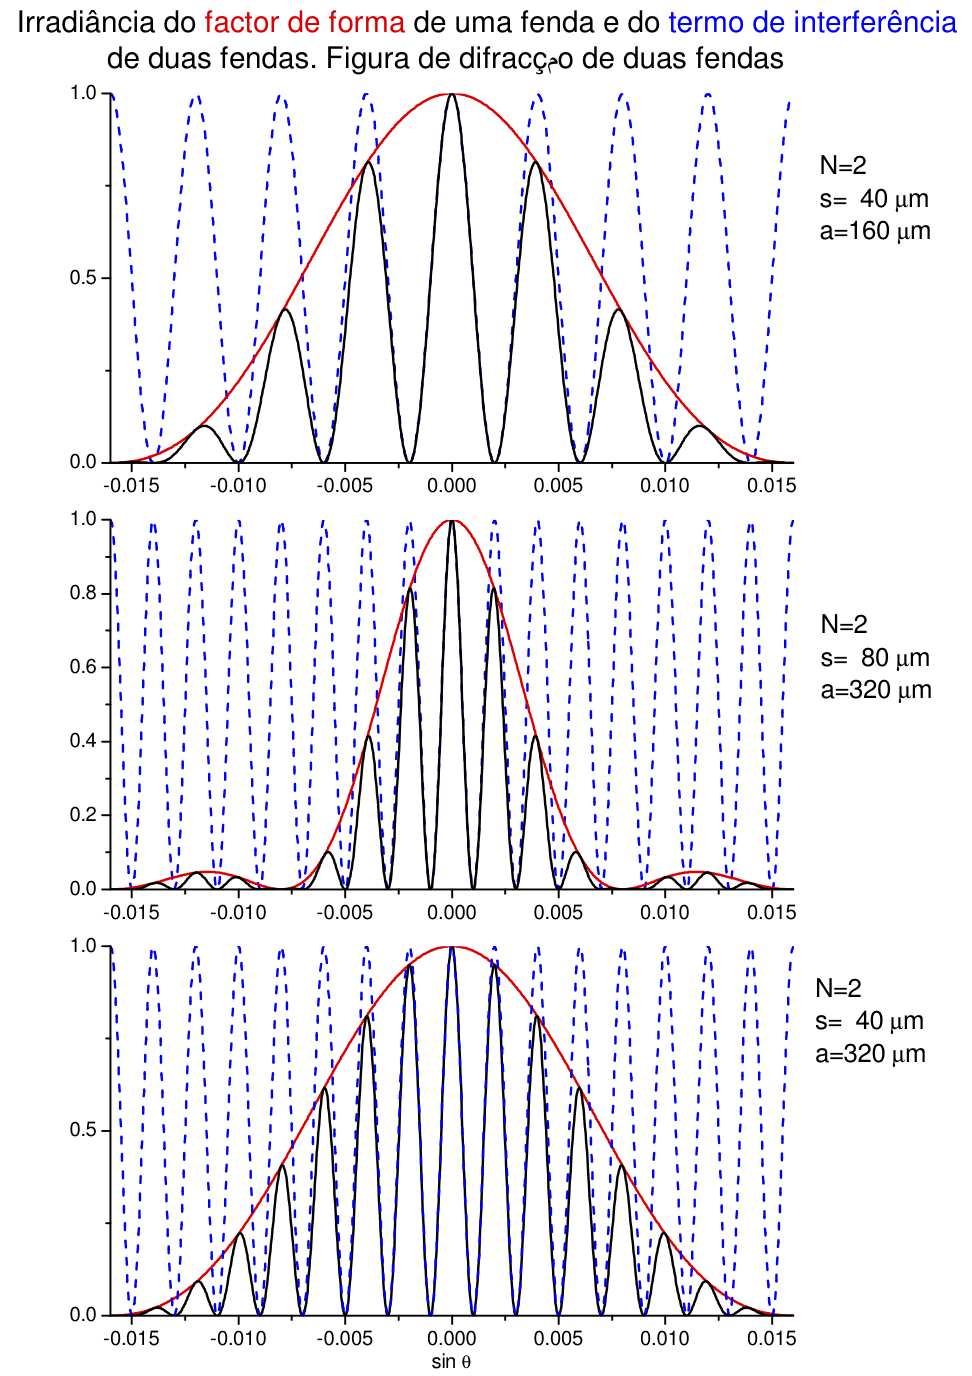
\includegraphics{./figura7}\label{fig:7} \\[1cm]  %%  Full page graphic
\end{center}



\begin{center}
	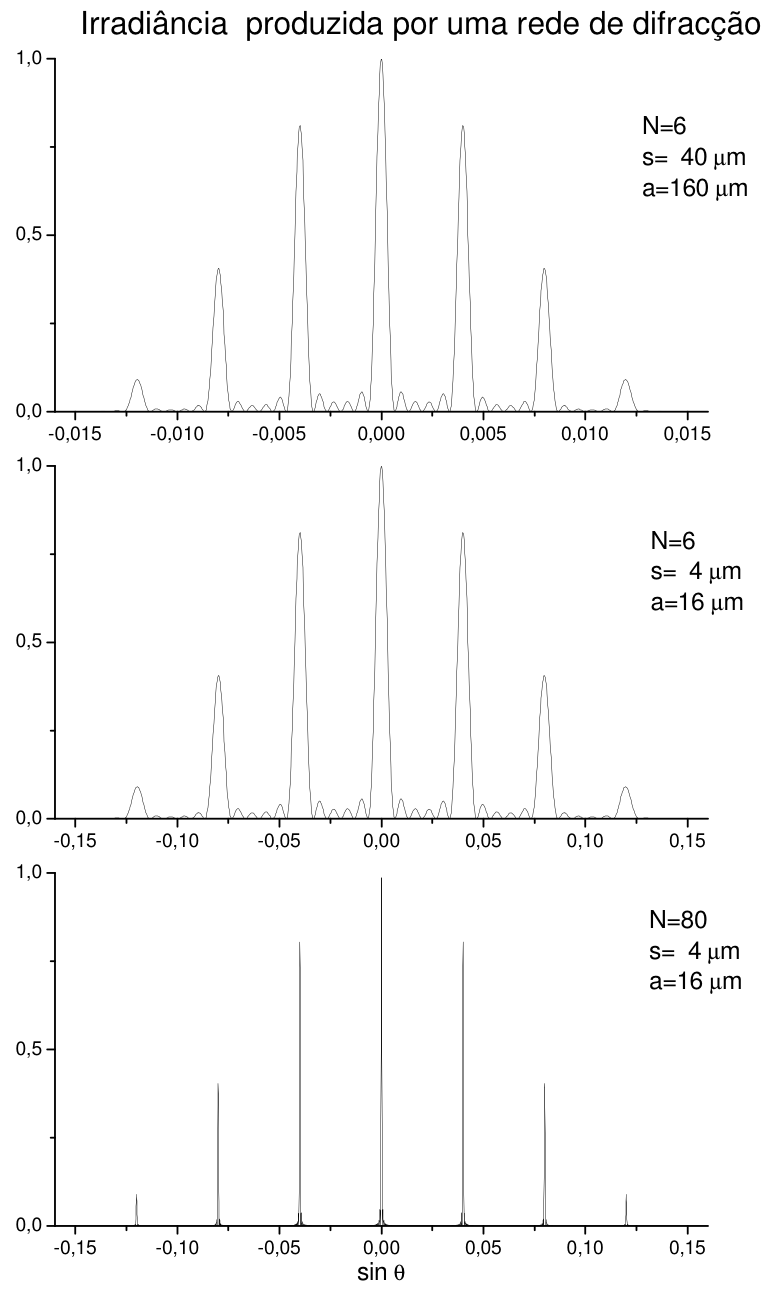
\includegraphics[width=0.8\textwidth]{figura8.png} \\ %[width=0.8\textwidth]
Para uma rede com um elevado número de linhas( no laboratório existem de 80, 100, 300 e 600 por mm) só são observáveis os máximos principais que correspondem a $\sin \theta =m\frac{\lambda}{a} $, notando-se o efeito do fator de forma da fenda que é uma envolvente da intensidade dos máximos.
\end{center}

%\begin{figure}[h!] \label{fig:8} \centering 
%	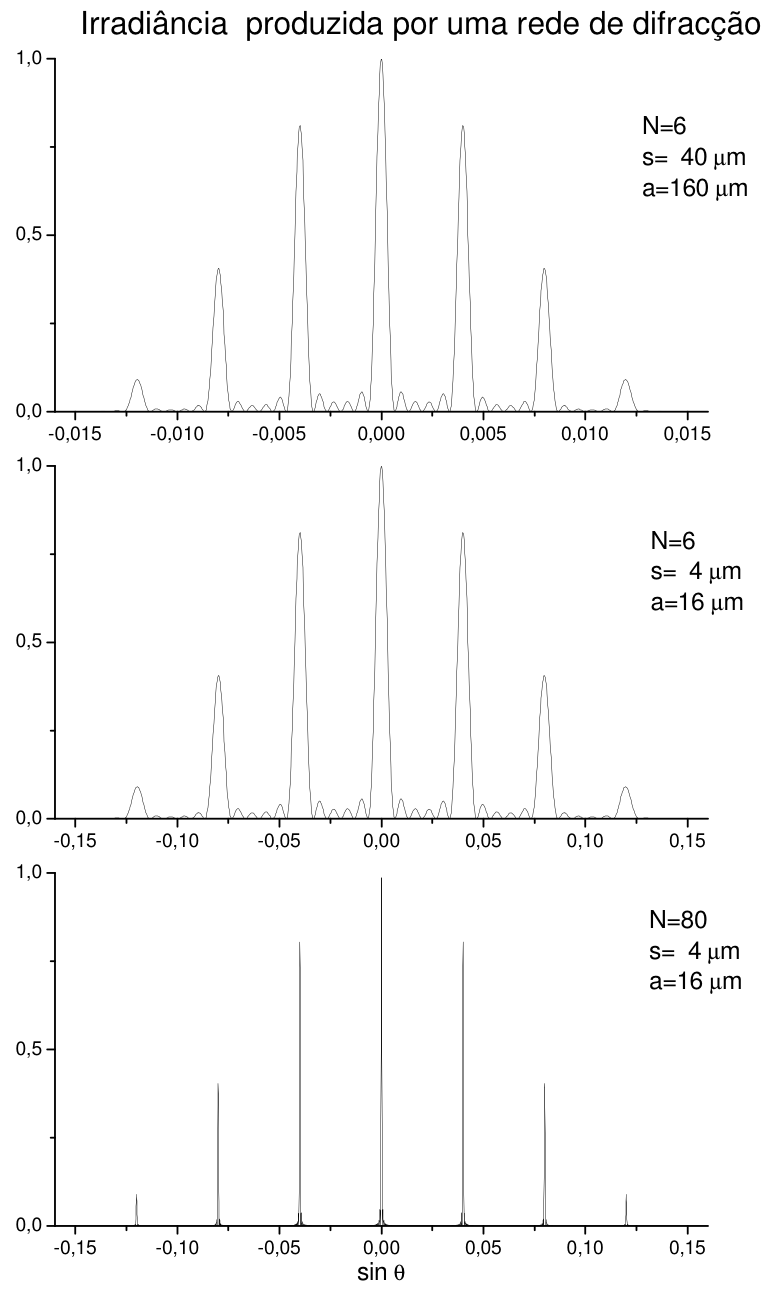
\includegraphics[width=0.8\textwidth]{figura8.png} 
%	\caption{Para uma rede com um elevado número de linhas( no laboratório existem de 80, 100, 300 e 600 por mm) %só são observáveis os máximos principais que correspondem a $\sin \theta =m\frac{\lambda}{a} $, notando-se o %efeito do fator de forma da fenda que é uma envolvente da intensidade dos máximos.} 
%\end{figure}


%\begin{verbatim}
%	10 PRINT "HELLO WORLD "; 20 GOTO 10 
%\end{verbatim}
%\pagebreak[3]

%%%%%%%%%%%%%%%%%%%%%%%
\section{Poder de Resolução de uma Rede de \mbox{Difração}}
Referiu-se, a propósito de resolução de um prisma, o critério de Rayleigh para resolução de duas riscas   como o afastamento mínimo dos dois comprimentos de onda associados  tal que o máximo de uma risca correspondia ao mínimo de outra (Figura \ref{fig:raleigh}). 

Devido ao termo de interferência  uma rede de $N$ fendas produz um máximo principal de ordem 1 ladeado do mínimo mais próximo, qual corresponde a 
 
 \begin{figure}
	[!tb]  \centering 
	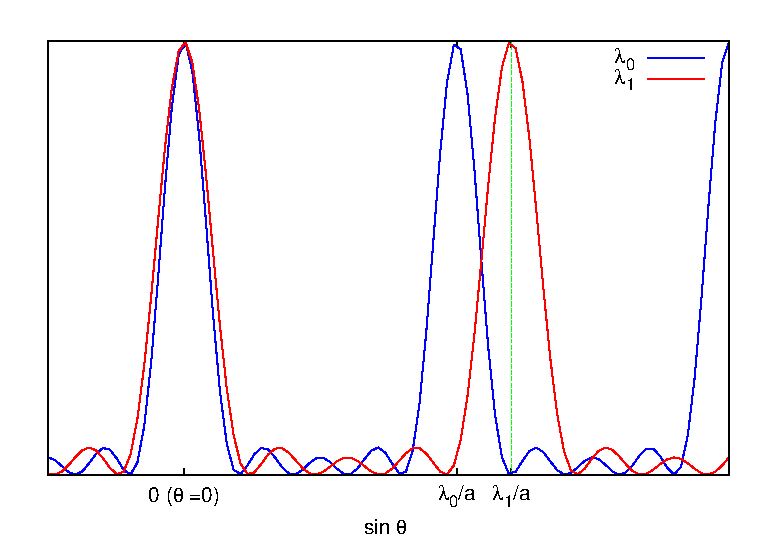
\includegraphics[width=0.7\textwidth]{raleigh} 
	\caption{Critério de resolução para uma rede de $N=5$ fendas, ordem $m=1$ e dois c.d.o.
	\label{fig:raleigh}} 
\end{figure}
%($\lambda_1 = \lambda_0 \frac{N+1}{N} $ )

\begin{equation*}
	|m'| = N + 1 \, \quad  \text{o que implica}  \,  v_{0_{min}}= \frac{m' \pi}{N} =  \frac{(N + 1)\pi}{N}
\end{equation*}
%\text{(pag. \pageref{eq:fendasminimos}),}

Assim o intervalo mínimo de $v$ que corresponde à diferença de posição do máximo para o mínimo seguinte será $\Delta v=  \dfrac{\pi}{N}$ o que atendendo a $ v = \dfrac{k a }{2} \sin \theta$
\begin{equation} \label{eq:50}
\frac{k a }{2} \cos \theta \Delta \theta = \frac{\pi}{N}
\end{equation}
em que $\Delta \theta$ é o intervalo angular correspondente ao critério de Rayleigh.

Se considerarmos agora que o feixe que incide na rede não é monocromático, uma variação de $\Delta \lambda$ em  
$\lambda$ produz uma variação angular $\Delta \theta$ que considerando a equação dos máximos da rede (\ref{eq:49}).
\begin{align} \label{eq:51}
 \frac{d}{d \theta} \left( \sin \theta \right) &=  
\frac{d}{d \theta} \left( m  \frac{\lambda}{a}\right) \\ 
\label{eq:52} \cos \theta &= \frac{m }{a} \frac{d \lambda}{d \theta} \Rightarrow 
\Delta \lambda = \frac{a \cos \theta}{m}  \Delta \theta 
\end{align}
 
Combinando (\ref{eq:52}) e (\ref{eq:50})  obtém-se para a \emph{resolução }$R$:
\begin{empheq}[box=\fcolorbox{blue!40!black!60}{yellow!20}]{equation}
	R = \frac{\lambda}{\Delta \lambda} = m N \label{eq:resolRede}
\end{empheq}
%\begin{equation}  \end{equation}

que depende apenas da ordem \underline{m} de difração e do número, $N$, de linhas (ou fendas) na rede de difração iluminadas pelo feixe .

%\newpage
\subsection{\sf Questões a responder ANTES da sessão de Laboratório:}
\begin{enumerate}
\item Dois altifalantes ligados ao mesmo canal de um amplificador estereofónico estão  separados de dois metros e emitem uma onda sonora de $f=1.0\,kHz$. Calcule o(s) ângulo(s) em relação à mediatriz que se deve colocar para deixar de ouvir o som. Explique porquê.
\item Se trocar a polaridade  dos fios a uma coluna o que acontece?
\item Um ponteiro Laser verde ($\lambda= 532\,nm$), é apontado a uma chapa com um “pinhole” de diâmetro $s=120\,\mu m$. Se tiver uma parede a
$150\,cm$ desta chapa que imagem irá observar? Justifique e faça um esboço à escala  1:1.
\end{enumerate}
\section{\sf Protocolo Experimental}

\subsection{\sf Material utilizado}
\begin{enumerate}
\item Caixa de Ótica equipada com calha graduada.
\item Slides com várias fendas, 
\item Redes de difração, filtros corados, suportes. 
\item Laser de He-Ne de potência $\le 5\, mW$.  
\item Detetor de intensidade luminosa linear tipo CCD e software de aquisição Caliens
\end{enumerate}

{\bf (Todas as figuras de difração obtidas devem ser incluídas no relatório)}

\subsection{\sf Difração por uma fenda}

\begin{enumerate}
\item Faça incidir numa das três fendas (A, B, C, respetivamente, 40, 80 e 160 µm) um 
feixe de luz monocromática proveniente de um laser de He-Ne ($\lambda=632.8\,nm$).  
Coloque o laser e o alvo, onde vai observar a figura, a distâncias tais que possa usar 
a aproximação de Fraunhofer (Justifique!). 
\item Estime a largura da fenda a partir da figura de difração obtida e da medição dos diversos mínimos (equação  \ref{eq:minF}).  
Repita pelo menos para duas posições diferentes do 
alvo.  
\item Estime a precisão e a exatidão que obteve nas duas situações. 
\item Difração por um cabelo: Repita  o  procedimento  do  ponto  anterior  usando  agora  um  cabelo  montado  num 
suporte.  
Estime a precisão obtida.  
Compare  a  figuras  de  difração  obtida  com  a  que  foi  registada  para  as  fendas  no 
ponto anterior, utilizando o \emph{Princípio de Babinet}.
\end{enumerate}

\subsection{\sf Difração por uma rede de $N$ linhas}
\begin{enumerate}
\item Faça incidir numa rede de Difração (de 80, 100 ou 600 linhas/mm) um 
feixe de luz do laser de He-Ne, ou outro laser de estado sólido (e.g. apontador laser).
\item A partir da medição dos máximos principais verifique a relação  (\ref{eq:maxRede}).
Estime a distância entre fendas e compare com o valor anunciado.
\item Estime o número de fendas iluminadas e indique quantos máximos e mínimos secundários (não visíveis...) que existem 
entre estes máximos principais.
\item Calcule a Resolução da rede nestas condições para a ordem $m=1$. 
\end{enumerate}


\subsection{\sf Difração por uma fenda dupla}

\begin{enumerate}
\item Faça incidir numa das três fendas duplas (D, E, F) um feixe de luz monocromática 
proveniente de um laser de He-Ne ($\lambda=632.8\,nm$).  
\item Usando um detetor CCD linear registe o perfil das intensidades com o programa instalado 
no PC ao qual o detetor está ligado. Conhecendo a largura de cada fenda ($s=40\, 
\mu m$ para D e E e $80\,\mu m$ para F), a distância entre fendas ($a=125\,\mu m$ para D e 
$250\,\mu m$  para  E  e  F) e a distância entre slide e alvo  simule  o  perfil  obtido  para  a  intensidade.  Guarde  o  ficheiro  das 
intensidades  em  formato  texto  para  poder  simular  o  perfil  usando  a  equação (\ref{eq:DF_s}) que 
permite calcular a intensidade da figura de difração, ajustando interativamente os parametros $s$ e $a$. 
\item Comente  o  que  observou  e  o  resultado  das  simulações  comparado  ao  perfil 
experimental. 
\end{enumerate}

\section{\sf Apêndice}
\subsection{Máximos da figura de difração de uma fenda} \label{sec:maxfenda}
Entre mínimos regularmente espaçados em $\sin \theta $ ocorrem máximos secundários correspondentes às soluções da equação 
\begin{equation}
	\label{eq:35} \frac{d}{d u} \left( \frac{\sin u}{u} \right)^2 = 0 \text{ (com 2ª derivada} \le 0) 
\end{equation}
\begin{align}
	\label{eq:36} 2 \frac{\sin u}{u} \frac{u \cos u- \sin u}{u^2} &= 0 \Rightarrow u \ne 0 \land u \cos u- \sin u =0\nonumber \\
	\tan u &= u 
\end{align}

%A evolução da função $\left( \frac{\sin u}{u} \right)^2 $ apresenta-se na figura \ref{fig:4} (a preto). Para se visualizarem os máximos secundários %apresenta-se a vermelho no mesmo gráfico com a escala de ordenadas $10$ vezes superior.


%\newpage 
As soluções da equação trigonométrica (\ref{eq:36}) que correspondem aos máximos secundários são calculados graficamente a partir do pontos de interseção de $\tan u$ com a reta $y=u$ (os Pontos $A$, $B$, $C$, $D$, etc.) que correspondem a valores $u$ menores mas próximos de $\frac{(2\,n +1)\pi}{2}$ com $n=1,\,2 \cdots$. 
\begin{figure}
	[htb] \label{fig:5} \centering 
	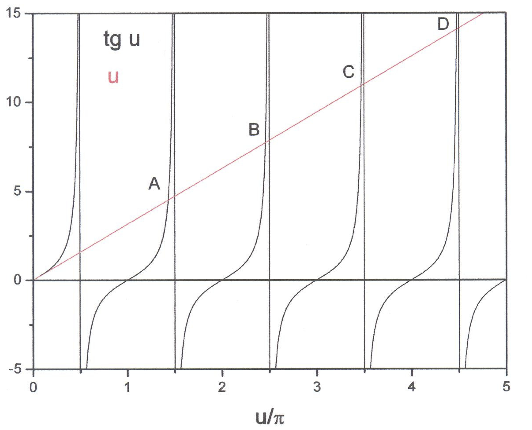
\includegraphics[width=0.7\textwidth]{figura5.png} \caption{ } 
\end{figure}
\begin{equation*}
	I(\frac{3\pi}{2}) =\frac{I_0}{(\frac{3\pi}{2})^2} \simeq 0.045 \, I_0 \qquad I(\frac{5\pi}{2}) \simeq 0.016 \, I_0 
\end{equation*}
As soluções numéricas são $u=\pm 1.4303\pi$ ; $\pm 2.45908\pi$, etc. e não $1.5\pi, \; 2.5\pi \cdots$ 

\subsection{Mínimos e Máximos Secundários da figura de difração de N fendas, afastadas de $a$}
\label{sec:maxminNfendas}
\subsubsection{Mínimos Secundários}

Quando $N v = m' \pi$, $v= \frac{m'}{N } \pi$ para $m' \ne m N$ o termo de interferência terá mínimos de intensidade.
%Mas quando $N v = m' \pi$, $v= \frac{m'}{N } \pi$ que não é necessariamente um múltiplo de $\pi$, pois em geral $\frac{m'}{N} \ne$inteiro,
%%%i.e. o termo de interferência, 
%para  $N v = m \pi$ será do tipo $\frac{0}{\ne 0}=0$ i.e. terá mínimos de intensidade para $N v = m \pi$. 
E quantos mínimos?
   
\begin{equation*}
	\label{eq:fendasminimos}
	m' =1, \cdots, N-1, N  \quad \rightarrow \quad \frac{m'}{N} = \underbrace{\frac{1}{N}, \cdots  \frac{N-1}{N}}_{N-1 \text{ valores } \ne \text{ inteiros}} , \frac{N}{N}
\end{equation*}

Difração por N Fendas de Largura s Afastadas de a
Haverá  portanto $N-1$ mínimos entre os máximos principais. 
\subsubsection{Máximos Secundários}
Entre estes mínimos haverá naturalmente máximos secundários, um entre cada dois mínimos consecutivos sendo portanto $N-2$, cujas posições podem ser calculados por
\begin{align}
	\frac{d}{d v} \big( \frac{\sin N v }{N \sin v} \big)^2 &= 2 \big( \frac{\sin N v }{N \sin v} \big)
	 \frac{N^2 \sin v \cos N v - N \sin N v \cos v }{N^2 \sin^2 v} \nonumber \\
	&= 2 \big( \frac{\sin N v }{N \sin v} \big)  \frac{N \cos N v \cos v}{N^2 \sin v}
	\big( N\frac{\sin v}{\cos v}  - N\frac{\sin N v}{\cos N v} \big) = 0 \nonumber \\
	&\Rightarrow \sin v \ne 0 \land N \tan v =  \tan Nv \label{eq:47}
\end{align}

Pode verificar-se que se trata de um máximo fazendo a 2ª derivada.


\end{document} 

